\documentclass[letterpaper,12pt,fleqn]{article}
\usepackage{matharticle}
\usepackage{tikz}
\pagestyle{empty}
\newcommand{\e}{\epsilon}
\renewcommand{\d}{\delta}
\begin{document}

\section*{Limit of a Function}

What is the behavior of a function \(f(x)\) as \(x\) gets arbitrarily close to some value \(c\)?

\bigskip

\begin{tikzpicture}
  \draw [thick] (-1,0) to (10,0);
  \draw [thick] (0,-1) to (0,5);
  \draw (-0.5,0) [out=80, in=180] to (1,3) [out=0, in=135] to (2,2.5)
        [out=-45,in=180] to (5,4) [out=0,in=180] to (8,3) [out=0,in=-100] to (10,5) node [right] {\(f(x)\)};
  \draw [dashed] (5,0) to (5,5);
  \node [below] at (5,0) {\(c\)};  
\end{tikzpicture}

In particular, does \(f(x)\) get arbitrarily close to some value \(L\) as \(x\) gets arbitrarily close to \(c\) from both
directions (left and right), regardless of whether or not \(c\) is in the domain of \(f(x)\)?  If so, then we call \(L\) the
\emph{limit} of \(f(x)\) as \(x\) approaches \(c\):
\[\lim_{x\to c}f(x)=L\]
This is essentially the book definition; however, we need something a little more analytical to see what this really means:
\begin{enumerate}
  \item Assume that we know that \(f(x)=L\).

    \begin{tikzpicture}
      \draw [thick] (-1,0) to (10,0);
      \draw [thick] (0,-1) to (0,5);
      \draw (-0.5,0) [out=80, in=180] to (1,3) [out=0, in=135] to (2,2.5)
            [out=-45,in=180] to (5,4) [out=0,in=180] to (8,3) [out=0,in=-100] to (10,5) node [right] {\(f(x)\)};
      \draw [dashed] (5,0) to (5,5);
      \node [below] at (5,0) {\(c\)};
      \draw [dashed,green] (0,4) -- (10,4);
      \node [left,green] at (0,4) {\(L\)};
    \end{tikzpicture}
    
  \item Assume \(\e>0\):

    \begin{tikzpicture}
      \draw [thick] (-1,0) to (10,0);
      \draw [thick] (0,-1) to (0,5);
      \draw (-0.5,0) [out=80, in=180] to (1,3) [out=0, in=135] to (2,2.5)
            [out=-45,in=180] to (5,4) [out=0,in=180] to (8,3) [out=0,in=-100] to (10,5) node [right] {\(f(x)\)};
      \draw [dashed] (5,0) to (5,5);
      \node [below] at (5,0) {\(c\)};
      \draw [dashed,green] (0,4) -- (10,4);
      \node [left,green] at (0,4) {\(L\)};
      \draw [dashed,red] (0,4.5) -- (10,4.5);
      \draw [dashed,red] (0,3.5) -- (10,3.5);
      \node [left,red] at (0,4.5) {\(L+\e\)};
      \node [left,red] at (0,3.5) {\(L-\e\)};
    \end{tikzpicture}

  \item Select some \(\d>0\) so that for all \(\abs{x-c}<\d\) all the \(f(x\) values are contained in the resulting box:

    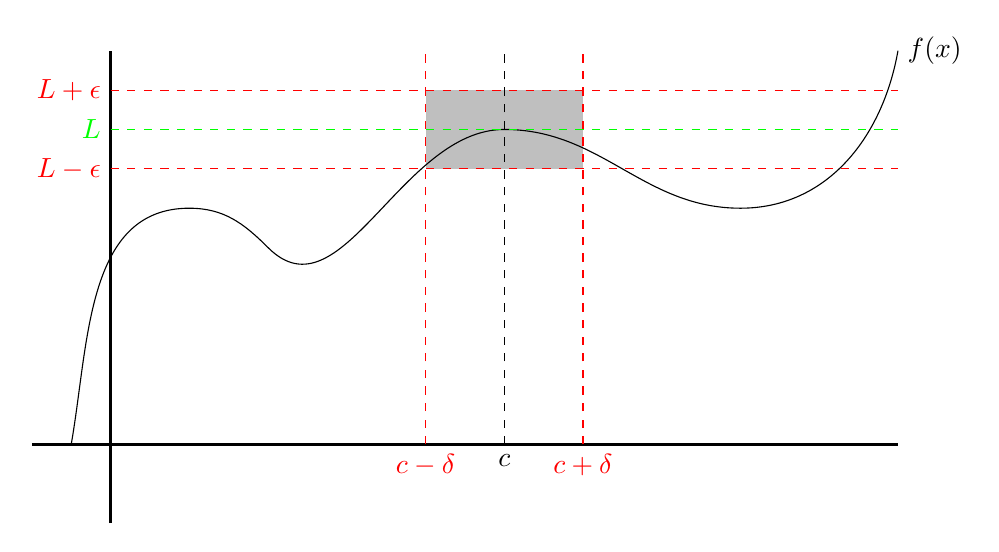
\begin{tikzpicture}
      \draw [thick] (-1,0) to (10,0);
      \draw [thick] (0,-1) to (0,5);
      \fill [lightgray] (4,3.5) rectangle (6,4.5);
      \draw (-0.5,0) [out=80, in=180] to (1,3) [out=0, in=135] to (2,2.5)
            [out=-45,in=180] to (5,4) [out=0,in=180] to (8,3) [out=0,in=-100] to (10,5) node [right] {\(f(x)\)};
      \draw [dashed] (5,0) to (5,5);
      \node [below] at (5,0) {\(c\)};
      \draw [dashed,green] (0,4) -- (10,4);
      \node [left,green] at (0,4) {\(L\)};
      \draw [dashed,red] (0,4.5) -- (10,4.5);
      \draw [dashed,red] (0,3.5) -- (10,3.5);
      \node [left,red] at (0,4.5) {\(L+\e\)};
      \node [left,red] at (0,3.5) {\(L-\e\)};
      \draw [dashed,red] (4,0) to (4,5);
      \draw [dashed,red] (6,0) to (6,5);
      \node [below,red] at (4,0) {\(c-\d\)};
      \node [below,red] at (6,0) {\(c+\d\)};
    \end{tikzpicture}
\end{enumerate}

Note that as \(\e\to0\), this forces \(\d\to0\) and the box converges on the limit \(L\).  This happens regardless of whether
\(x=c\) is in the domain of \(f(x)\) or not, since \(\d>0\) and thus \(x\ne c\).

The functions that we are going to look at are fairly well-behaved and so finding limits by visualization and a few
simple rules will be sufficient.

\begin{examples}
  Let's start with some visual examples: p549 \#1--4.
\end{examples}

But where might there fail to be some limit of a function as \(x\) approaches some point \(c\)?
\begin{enumerate}
\item Gaps
  \[f(x)=\frac{x}{\abs{x}}, c=0\]

\item Breaks
  \[f(x)=\frac{1}{x}, c=0\]
\end{enumerate}
You can always find an \(\e\) for which no suitable \(\d\) exists.

\begin{examples}
  p552 \#66--70.
\end{examples}

Now, lets see how to analytically find limits for some of our basic functions (Section 2.5 p215).

\end{document}
